\documentclass[11pt,a4paper]{article}

\usepackage[utf8]{inputenc}
\usepackage[T1]{fontenc}
\usepackage[margin=2.5cm]{geometry}
\usepackage{amsmath,amssymb}
\usepackage{bm}
\usepackage{graphicx}
\usepackage{booktabs}
\usepackage{caption}
\usepackage{hyperref}

\graphicspath{{figures/}}

\newcommand{\Rea}{\operatorname{Re}}
\newcommand{\Ima}{\operatorname{Im}}

\title{Tracking the Floquet branch with harmonic modal participation:\\
the damped Mathieu ODE and the flapwise ODE of a rotor blade}
\author{}
\date{}

\begin{document}
\maketitle

\begin{abstract}
The imaginary part of a Floquet characteristic exponent is only defined up to integer
multiples of the excitation frequency. Choosing the correct branch requires an addition
factor $m$. This note examines whether a modal analysis of the Floquet mode, i.e.\ the
harmonic participation of its periodic part, can identify the switches between branches
and thereby the addition factor. The analysis is carried out for the damped Mathieu ODE
and for the flapwise ODE of a single rotor blade in rotating coordinates. In both cases,
the switches of the dominant harmonic and the peaks of the participation gap at low
parameter values, and the peaks of the participation-weighted (centroid) frequency at
higher parameter values, coincide with the branch switches obtained from the
characteristic multipliers. The addition factor reconstructed from the modal analysis is
identical, as an integer, to the multiplier-based addition factor over the complete
parameter ranges. At the same time, the dominant harmonic content of the mode does not
follow the tracked exponent at high parameter values; the reasons and the resulting
limitations are discussed.
\end{abstract}

%-------------------------------------------------------------------------------
\section{Objective}
For a linear system with periodic coefficients, $\dot{\bm{x}} = \bm{A}(\psi)\,\bm{x}$ with
$\bm{A}(\psi + T) = \bm{A}(\psi)$, $T = 2\pi$ and $\Omega = 1$, the characteristic
exponents follow from the characteristic multipliers $\lambda_i$, the eigenvalues of the
monodromy matrix $\bm{\Phi}(T)$:
\begin{equation}
  s_i = \frac{1}{T}\ln \lambda_i = \sigma_i + \mathrm{i}\,\omega_i ,
  \qquad
  \omega_i = \omega_{i,0} + m\,\Omega, \quad m \in \tfrac{1}{2}\mathbb{Z}.
  \label{eq:floquet}
\end{equation}
The real part $\sigma_i$ is unique, the imaginary part is not: the principal value
$\omega_{i,0}$ has to be complemented by an addition factor $m$. The question addressed
here is whether the harmonic content of the Floquet mode indicates where the branch, and
hence $m$, changes, independently of the ordering of the multipliers.

%-------------------------------------------------------------------------------
\section{Method}

\paragraph{Monodromy matrix and reference addition factor.}
$\bm{\Phi}(\psi)$ is integrated with \texttt{ode45} from $\bm{\Phi}(0) = \bm{I}$. The
reference addition factor $m_\lambda$ is obtained from the multipliers:
\begin{itemize}
  \item Mathieu ODE: $m_\lambda$ starts at 0 and increases by $\tfrac{1}{2}$ whenever a
        resonance ``bubble'' opens, i.e.\ when the two real parts $\sigma_1 \neq \sigma_2$
        split because the multipliers become real.
  \item Flapwise ODE: the multipliers are sorted by their real part (complex-conjugate
        pairs with the negative imaginary part first),
        $\sigma = \ln|\lambda|/T$ and $\omega_0 = \arctan(\Ima\lambda/\Rea\lambda)/T$, as in
        \texttt{BerechnungSchlagDGL.m}. $m_\lambda$ starts at 1, since the flap frequency
        starts near 1/rev, and increases by $\tfrac{1}{2}$ whenever the order of the
        magnitudes $|\lambda_1|$, $|\lambda_2|$ flips. The real parts are corrected by
        mirroring the larger one about its value at $\mu = 0$; the tracked frequency is
        $\omega_\text{track} = \omega_0 + m_\lambda$.
\end{itemize}

\paragraph{Harmonic modal participation.}
For the selected exponent $s$ with eigenvector $\bm{v}$ of $\bm{\Phi}(T)$, the periodic
part of the Floquet mode is
\begin{equation}
  \bm{P}(\psi) = \bm{\Phi}(\psi)\,\bm{v}\,\mathrm{e}^{-s\psi}, \qquad \bm{P}(\psi + T) = \bm{P}(\psi).
\end{equation}
Its displacement component $q(\psi)$ is expanded in harmonics $c_k$ (FFT over one period),
$k \in K = \{-4, \dots, 4\}$. With the participation and the branch frequencies
\begin{equation}
  \phi_k = \frac{|c_k|}{\sum_{j\in K}|c_j|}, \qquad \omega_k = |k + \Ima s| ,
\end{equation}
three frequencies are compared with $\omega_\text{track}$ (Mathieu: $\Ima s_{R1}$):
the dominant-branch frequency $\omega(\phi_\text{max}) = \omega_{k^*}$ with
$k^* = \arg\max_k \phi_k$, and the centroid frequency
$\omega_\text{mean} = \sum_{k} \phi_k\,\omega_k$. The participation gap $\Delta$ is the
change between neighbouring parameter values of the difference between the two largest
participations; its peaks mark changes of the dominant harmonic.

\paragraph{Modal addition factor.}
The addition factor after Peters, $m_P$, is reconstructed from the modal analysis only:
\begin{equation}
  m_P = m_0 + \tfrac{1}{2}\,[\text{first peak of } \Delta,\ \text{only if } m_0 = 0]
        + \tfrac{1}{2}\,\#\{\text{peaks of } \omega_\text{mean}\},
\end{equation}
with the start value $m_0 = 0$ (Mathieu) and $m_0 = 1$ (flap). For the comparison, integer
addition factors $\lfloor m \rfloor$ are used.

%-------------------------------------------------------------------------------
\section{Damped Mathieu ODE}
\begin{equation}
  \ddot{x} + 2D\dot{x} + \left(\nu_0^2 + \nu_c^2\cos\psi\right)x = 0, \qquad
  D = 0.15, \quad \nu_0^2 = \nu_c^2 = \nu \in [0, 9]
\end{equation}
(500 parameter values, $N_\text{FFT} = 2048$, mode with positive imaginary part).
Figure~\ref{fig:mathieu} shows the results.

\begin{figure}[htbp]
  \centering
  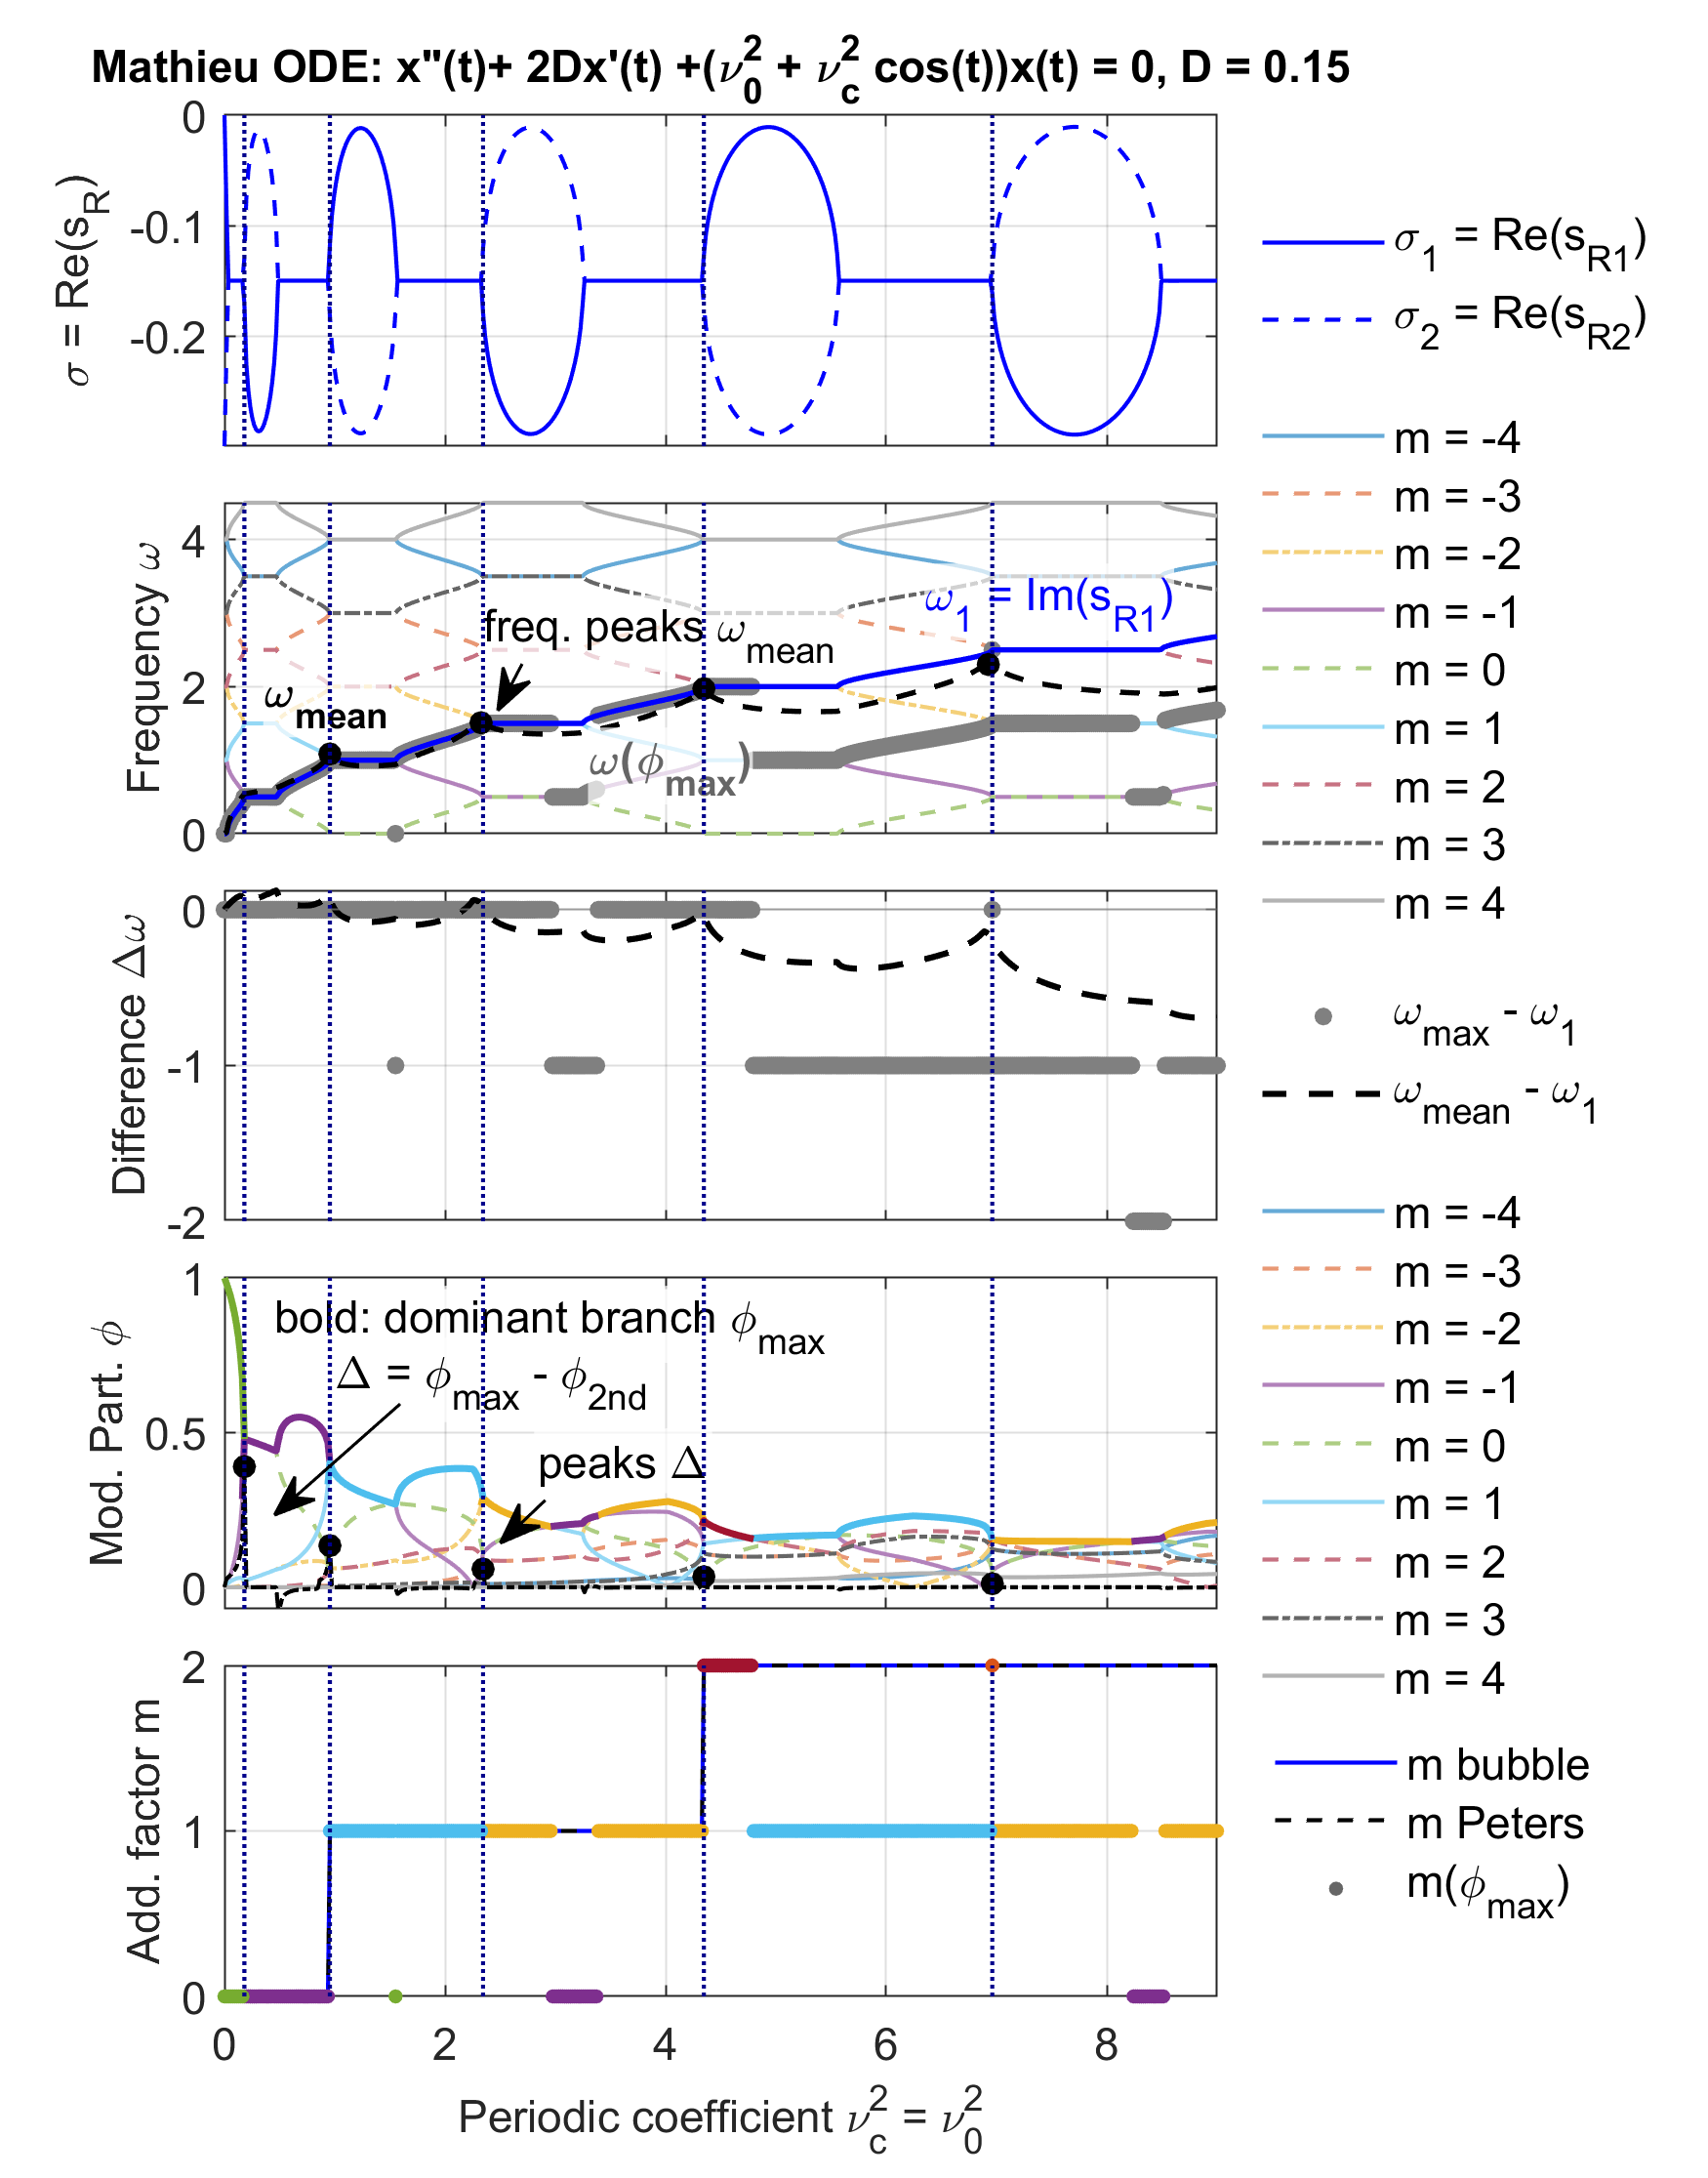
\includegraphics[width=0.78\textwidth]{mathieu_combined.png}
  \caption{Damped Mathieu ODE, $D = 0.15$, $\nu_0^2 = \nu_c^2$. From top: real parts of both
  exponents; branch frequencies $\omega_k$ with $\Ima s_{R1}$ (blue), $\omega_\text{mean}$
  (dashed, peaks as dots) and $\omega(\phi_\text{max})$ (grey); differences to
  $\Ima s_{R1}$; participation $\phi_k$ with the dominant branch in bold and the gap
  $\Delta$; addition factors $\lfloor m_\lambda \rfloor$ (``m bubble''),
  $\lfloor m_P \rfloor$ (``m Peters'') and the value implied by the dominant branch.
  Vertical lines: bubble openings.}
  \label{fig:mathieu}
\end{figure}

\paragraph{Findings.}
\begin{itemize}
  \item Outside the bubbles both real parts equal $-D = -0.15$; inside, they split
        symmetrically about $-D$ (parametric resonance). Along $\nu_0^2 = \nu_c^2$ the
        system remains stable ($\max\sigma \approx -0.01$).
  \item Bubbles open at $\nu = 0.18,\ 0.96,\ 2.34,\ 4.35,\ 6.96$. The participation gap
        $\Delta$ peaks at all five openings, the centroid $\omega_\text{mean}$ peaks at the
        second to fifth opening ($\nu = 0.96,\ 2.33,\ 4.35,\ 6.93$).
  \item $\lfloor m_P\rfloor = \lfloor m_\lambda\rfloor$ over the whole range; the
        half-step values run from 0 to 2.5.
  \item The dominant branch switches at the openings ($k^* = 0 \to -1 \to +1 \to -2 \to +2$)
        and $\omega(\phi_\text{max}) = \Ima s_{R1}$ up to $\nu \approx 4.8$. Beyond, the
        dominant harmonic is one order lower over the whole remaining range.
  \item The centroid drifts below $\Ima s_{R1}$ between the openings
        ($\omega_\text{mean} - \Ima s_{R1} \approx -0.38$ at $\nu = 5.8$, $-0.69$ at
        $\nu = 9$) and returns to it at each opening. The largest participation decreases
        from 1 ($\nu = 0$) to 0.37 ($\nu = 1$), 0.19 ($\nu = 4.5$) and about 0.2 ($\nu = 9$).
\end{itemize}

%-------------------------------------------------------------------------------
\section{Flapwise ODE of a single blade in rotating coordinates}
\begin{equation}
  \ddot\beta + c(\psi)\,\dot\beta + k(\psi)\,\beta = 0,
\end{equation}
\begin{align}
  c(\psi) &= \frac{\gamma}{2}\left(d_4 + e_\beta d_3 + \mu d_3 \sin\psi\right), \\
  k(\psi) &= \nu_0^2 + \frac{\gamma}{2}\left(\mu\,(d_3 + e_\beta d_2)\cos\psi
             + \frac{\mu^2}{2}\,d_2 \sin 2\psi\right),
\end{align}
with the parameters of configuration 7 in \texttt{Parameter.xlsx}: $\gamma = 8.159$,
$\nu_0 = 1.117$, $e_\beta = 0.1527$, $d_2 = 0.3098$, $d_3 = 0.1784$, $d_4 = 0.111$.
The advance ratio is varied as $\mu \in [0, 10]$ in steps of 0.1 ($N_\text{FFT} = 4096$;
mode with the largest $|\lambda|$, for complex pairs the member with positive imaginary
part). At $\mu = 0$, $\sigma = -\bar c/2 = -0.282$ and
$\omega = \sqrt{\nu_0^2 - \bar c^{\,2}/4} = 1.081$. Figure~\ref{fig:flap} shows the results.

\begin{figure}[htbp]
  \centering
  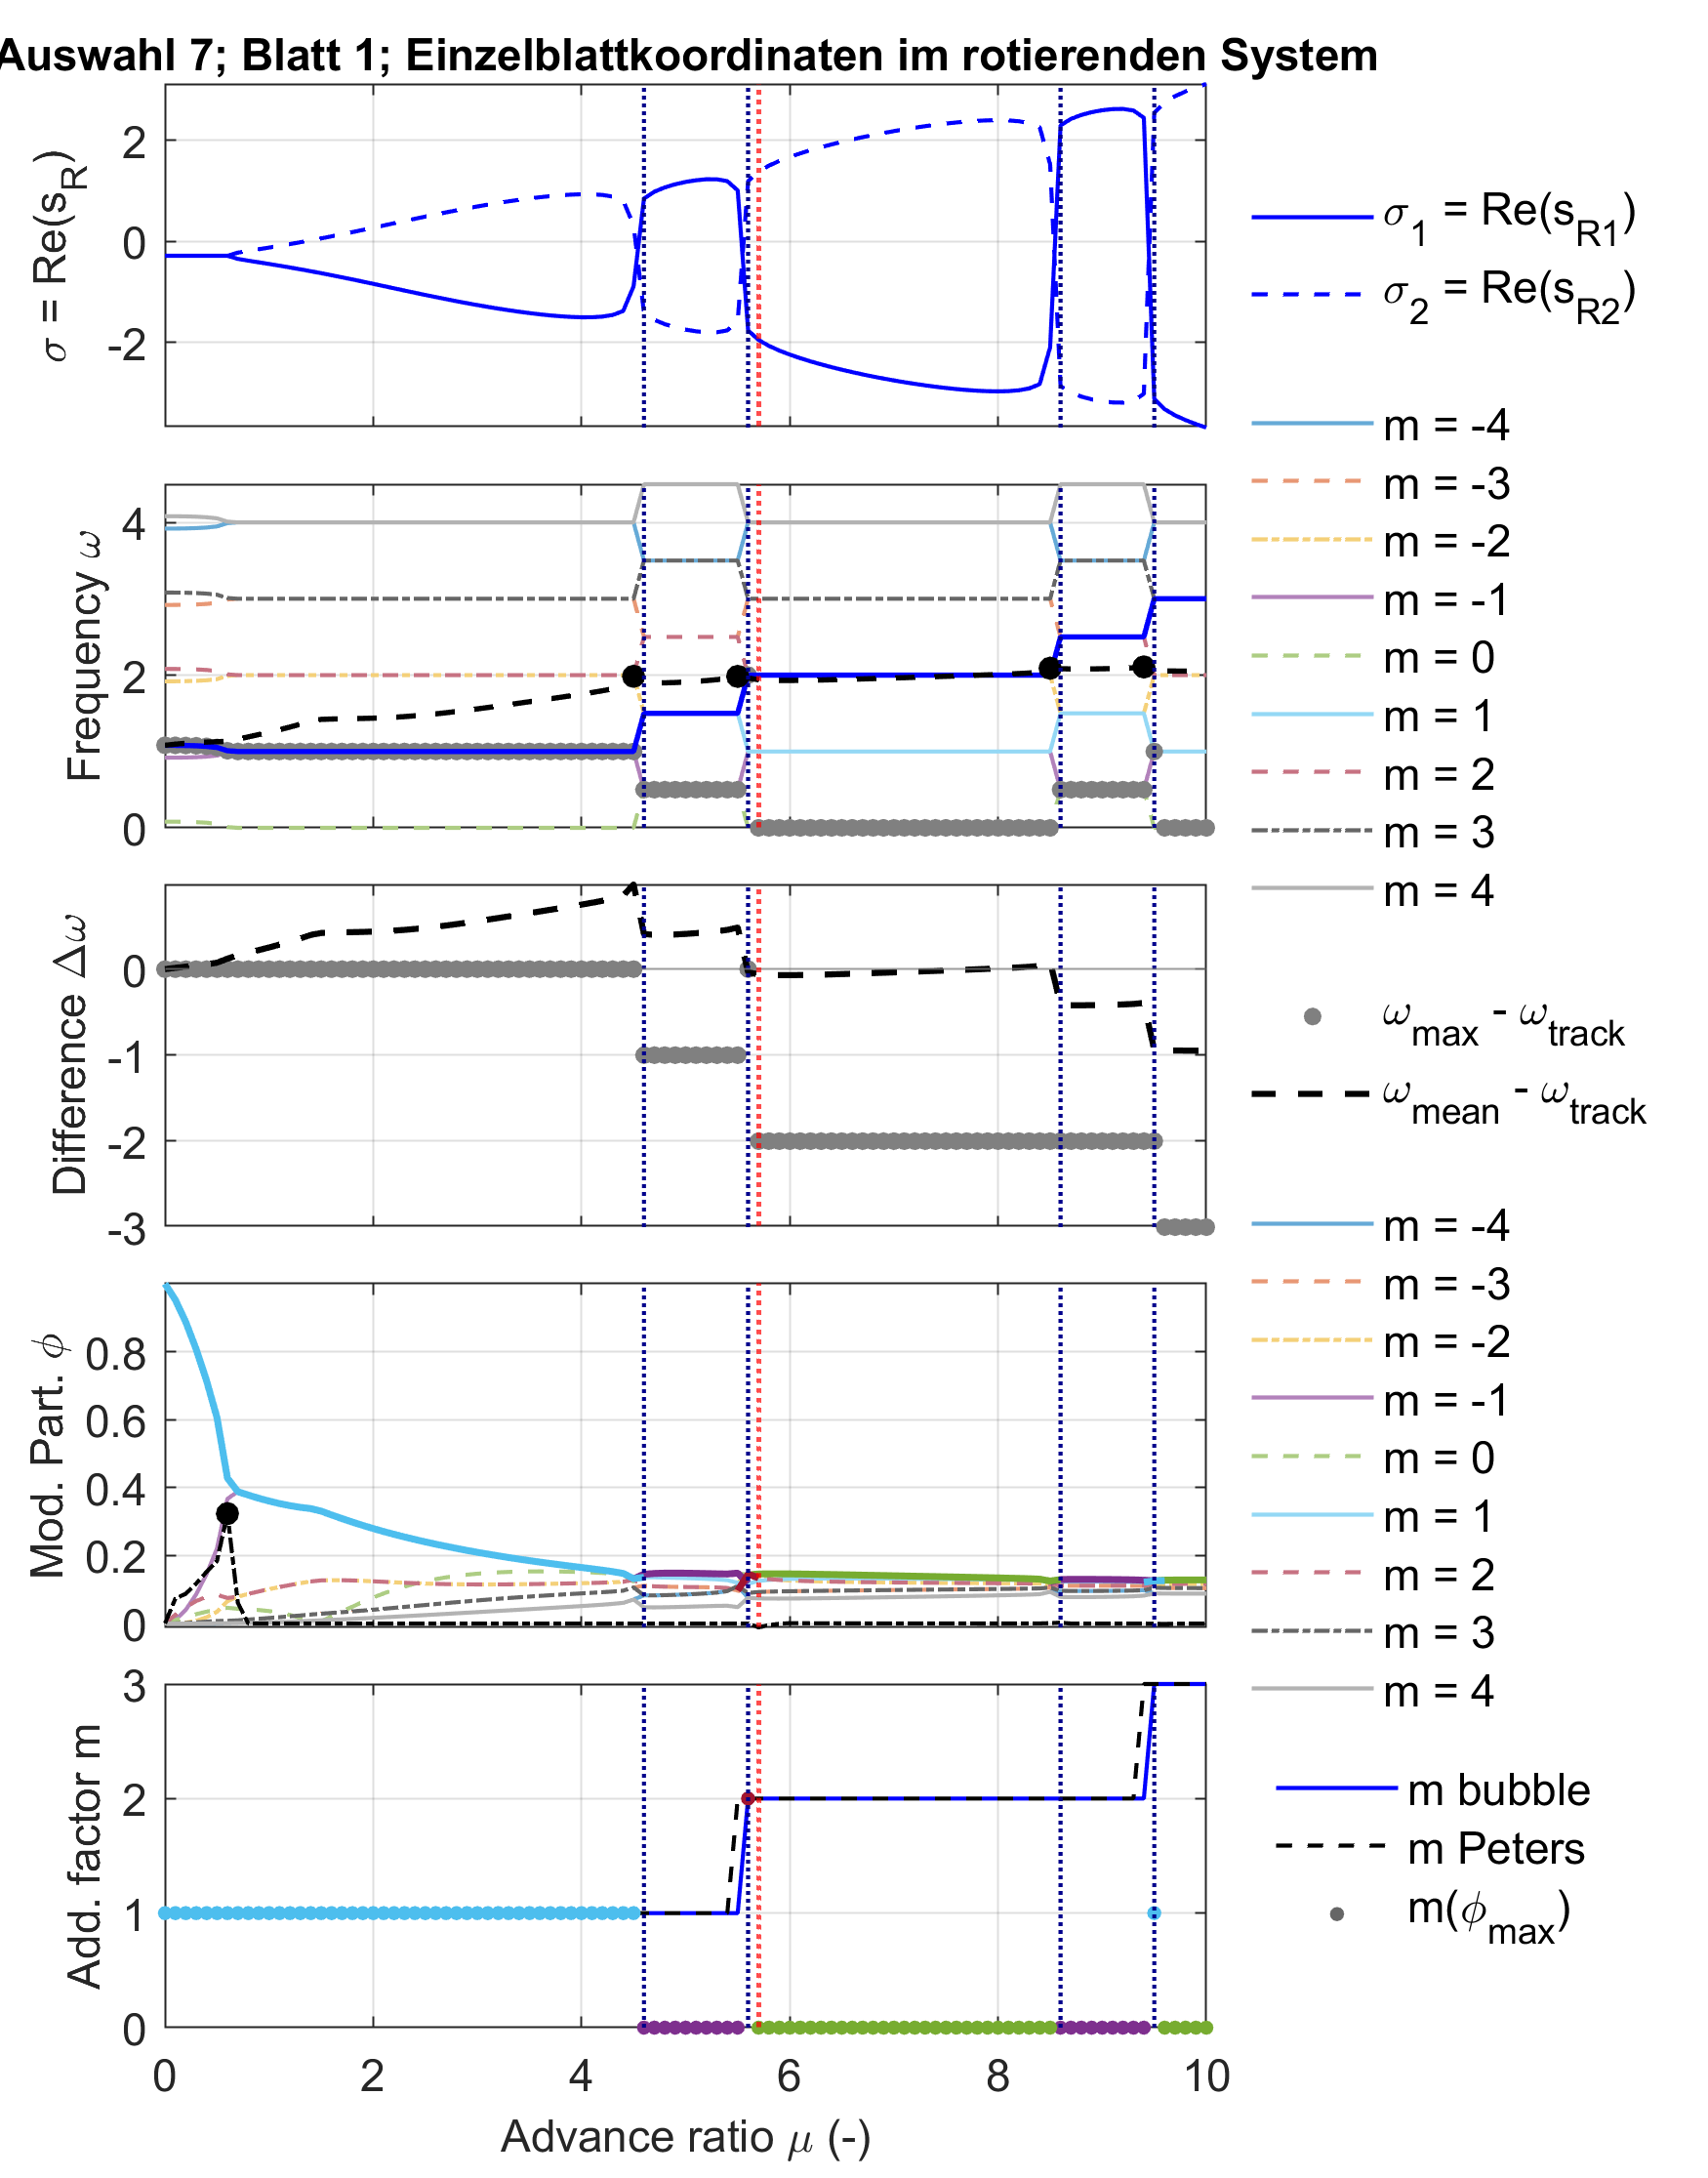
\includegraphics[width=0.78\textwidth]{flap_combined_Auswahl7.png}
  \caption{Flapwise ODE, single blade in rotating coordinates (configuration 7), versus
  advance ratio $\mu$. Panels as in Figure~\ref{fig:mathieu}, with
  $\omega_\text{track}$ (blue) as reference. Vertical dotted lines: changes of
  $m_\lambda$; red line: $\operatorname{cond}(\bm{\Phi}(T)) > 10^9$.}
  \label{fig:flap}
\end{figure}

\paragraph{Findings.}
\begin{itemize}
  \item The multipliers become real at $\mu \approx 0.6$--$0.7$; the frequency locks at
        1.0/rev. The order of the multiplier magnitudes flips at
        $\mu = 4.6,\ 5.6,\ 8.6,\ 9.5$, and $\omega_\text{track}$ steps through
        $1.0,\ 1.5,\ 2.0,\ 2.5,\ 3.0$. Real parts and $\omega_\text{track}$ agree with
        \texttt{BerechnungSchlagDGL.m} to machine precision.
  \item The participation gap $\Delta$ peaks once, at $\mu = 0.6$, where the frequency
        locks at the integer value 1 already contained in $m_0$. The centroid
        $\omega_\text{mean}$ peaks at $\mu = 4.5,\ 5.5,\ 8.5,\ 9.4$, i.e.\ one parameter
        step before each flip of the multiplier order.
  \item $\lfloor m_P\rfloor = \lfloor m_\lambda\rfloor$:
        $1 \to 2$ at $\mu \approx 5.5$--$5.6$ and $2 \to 3$ at $\mu \approx 9.4$--$9.5$.
  \item The dominant harmonic is $k^* = +1$ ($\omega = 1.0$) up to $\mu = 4.6$;
        $k^* = -1$ ($\omega = 0.5$, negative real multiplier, period $2T$) for
        $4.6 \le \mu < 5.6$ and $8.6 \le \mu < 9.5$; $k^* = 0$ ($\omega \approx 0$,
        positive real multiplier, non-oscillating mode) for $5.7 \le \mu < 8.6$ and
        $\mu \ge 9.5$. Hence $\omega(\phi_\text{max}) - \omega_\text{track} = 0, -1, -2, -2, -3$.
  \item The largest participation drops from 1 ($\mu = 0$) to 0.28 ($\mu = 2$) and to
        about 0.13 for $\mu \ge 4.5$; $\omega_\text{mean}$ settles at about 1.9--2.1.
  \item $\operatorname{cond}(\bm{\Phi}(T)) > 10^9$ for $\mu \ge 5.7$. The corrected real
        parts and the participation are computed from the dominant multiplier only.
\end{itemize}

%-------------------------------------------------------------------------------
\section{Summary of both cases}
Table~\ref{tab:summary} compares the branch switches obtained from the multipliers with
the events found by the modal analysis.

\begin{table}[htbp]
  \centering
  \caption{Branch switches from the multipliers and from the modal analysis.}
  \label{tab:summary}
  \small
  \begin{tabular}{p{0.27\textwidth}p{0.33\textwidth}p{0.33\textwidth}}
    \toprule
     & Mathieu ($D = 0.15$) & Flap (configuration 7) \\
    \midrule
    Switches from multipliers & $\nu = 0.18, 0.96, 2.34, 4.35, 6.96$ & $\mu = 4.6, 5.6, 8.6, 9.5$ \\
    Peaks of $\Delta$          & all five openings                     & $\mu = 0.6$ (lock at 1/rev) \\
    Peaks of $\omega_\text{mean}$ & $\nu = 0.96, 2.33, 4.35, 6.93$     & $\mu = 4.5, 5.5, 8.5, 9.4$ \\
    $\lfloor m_P\rfloor$ vs.\ $\lfloor m_\lambda\rfloor$ & identical & identical \\
    $\omega(\phi_\text{max})$ vs.\ tracked & equal up to $\nu \approx 4.8$, then $-1$ & equal up to $\mu = 4.6$, then $-1 \dots -3$ \\
    Largest participation at the end & $\approx 0.2$ & $\approx 0.13$ \\
    \bottomrule
  \end{tabular}
\end{table}

%-------------------------------------------------------------------------------
\section{Why the dominant harmonic does not rise for the flapwise ODE}
In the Mathieu sweep, $\nu_0^2 = \nu_c^2 = \nu$ increases the mean stiffness, so the
natural frequency $\sqrt{\nu_0^2}$ and with it the dominant harmonic rise. For the flapwise
ODE the mean coefficients over one revolution do not depend on the advance ratio,
\begin{equation}
  \bar c = \frac{\gamma}{2}\left(d_4 + e_\beta d_3\right) = 0.564, \qquad
  \bar k = \nu_0^2 = 1.248,
\end{equation}
because $\mu$ only scales the periodic terms. A control computation with the Mathieu ODE
confirms this (Table~\ref{tab:control}, script
\texttt{doc/mathieu\_fixed\_mean\_stiffness\_check.m}): with a fixed mean stiffness
$\nu_0^2 = 1$ the dominant frequency stays at 1/rev and then drops to 0 and 0.5/rev,
exactly as for the flapwise ODE.

\begin{table}[htbp]
  \centering
  \caption{Frequency of the dominant harmonic $\omega(\phi_\text{max})$ of the Mathieu
  ODE ($D = 0.15$) for a growing and for a fixed mean stiffness.}
  \label{tab:control}
  \begin{tabular}{lcccccccccc}
    \toprule
    $\nu$ & 0.05 & 1 & 2 & 3 & 4 & 5 & 6 & 7 & 8 & 9 \\
    \midrule
    $\nu_0^2 = \nu_c^2 = \nu$         & 0.17 & 1 & 1.3 & 0.5 & 1.8 & 1 & 1.2 & 1.5 & 1.5 & 1.7 \\
    $\nu_0^2 = 1$, $\nu_c^2 = \nu$    & 0.99 & 1 & 1   & 0   & 0   & 0 & 0   & 0   & 0   & 0.5 \\
    \bottomrule
  \end{tabular}
\end{table}

Consequently, the increasing addition factor of the flapwise ODE describes the continuity
of the Floquet branch (locking of $\omega$ at multiples of $\tfrac{1}{2}$ and the flips of
the multiplier order), not an increase of the frequency content of the blade motion.

%-------------------------------------------------------------------------------
\section{Assessment and limitations}

\paragraph{Supported.} In both ODEs the modal analysis detects the branch switches of the
Floquet exponent without using the ordering of the multipliers: at low parameter values
by switches of the dominant branch and peaks of the participation gap, at higher values
by peaks of the centroid frequency. The addition factor reconstructed from these events
coincides, as an integer, with the multiplier-based addition factor over the complete
parameter ranges.

\paragraph{Limitations.}
\begin{enumerate}
  \item \emph{Location, not value.} The modal analysis locates a switch; the step of
        $\tfrac{1}{2}$, the start value $m_0$ and the rule that the first lock of the
        flap mode at the integer value 1 adds no step are prescribed.
  \item \emph{Physical meaning of the tracked frequency.} The dominant harmonic content
        follows the tracked exponent only up to $\nu \approx 4.8$ (Mathieu) and
        $\mu \approx 4.6$ (flap). The modal analysis therefore supports a consistent,
        continuous branch choice; it does not show that the tracked frequency is the
        frequency at which the system predominantly oscillates.
  \item \emph{Robustness.} At high parameter values the participation is spread over
        many harmonics ($\phi_\text{max} \lesssim 0.15$ for the flap), and
        $\omega_\text{mean}$ is partly determined by the truncation $K = \{-4,\dots,4\}$.
        The centroid peaks are small cusps detected on a grid of 0.1 in $\mu$. Checks with
        a wider harmonic range, a finer parameter step and a different $N_\text{FFT}$ are
        recommended before generalising.
  \item \emph{Numerical conditioning.} For $\mu \ge 5.7$, $\operatorname{cond}(\bm{\Phi}(T))
        > 10^9$; only the dominant multiplier is resolved accurately, which is the one
        used here.
  \item \emph{Mode selection.} For complex-conjugate pairs the two members have mirrored
        spectra ($k \leftrightarrow -k$). The choice of the member changes the label of the
        dominant harmonic, not the frequencies.
\end{enumerate}

\paragraph{Suggested statement.} \emph{Harmonic modal participation analysis identifies
the parameter values at which the Floquet branch switches, both for the damped Mathieu
ODE and for the flapwise ODE. The addition factor reconstructed from these switches
coincides with the multiplier-based addition factor, which makes it possible to track a
consistent characteristic exponent including its addition factor.}

%-------------------------------------------------------------------------------
\section{Reproduction}
\begin{itemize}
  \item Mathieu ODE: \texttt{Mathieusche Differentialgleichung/Programme/compareImagCharExpFreqParticipation\_OnePlot.m}
  \item Flapwise ODE: \texttt{Schlagdifferentialgleichung/Programme/RotorFloquet\_Combined\_Auswahl7.m}
        (reference: \texttt{BerechnungSchlagDGL.m})
  \item Control computation: \texttt{doc/mathieu\_fixed\_mean\_stiffness\_check.m}
\end{itemize}

\end{document}
